\section{Monday 10/28/2024}
\subsection{Nesterov's optimal method}

\begin{algorithm}
  \caption{Nesterov's Method}\label{euclid}
  \begin{algorithmic}[1]
  \State $\textbf{y}^1 = \textbf{x}^0 \in \mathbb{R}^n, t_1 = 1, k = 1$
  \For {$ k = 1, \dots, K$}
    \State $\textbf{x}^k = \textbf{y}^k - \frac{1}{L} \nabla f(\textbf{y}^k)$
    \State $t_{k+1} = \frac{1+ \sqrt{1+4t_k^2}}{2}$
    \State $y^{k+1} = x^k + \frac{t_k-1}{t_{k+1}}(x^k - x^{k-1})$
    \State $k += 1$
  \EndFor
  \end{algorithmic}
\end{algorithm}
\subsection{Alternative Gradient Descent}
Alternative intepretation of gradient Descent
\begin{equation}
  \textbf{x}^k = \argmin_x f(\textbf{x}^{k-1}) + \langle \nabla f(\textbf{x}^{k-1}), \textbf{x} - \textbf{x}^{k-1} \rangle  + \frac{1}{2 \alpha^k} \| \textbf{x} - \textbf{x}^{k-1}\|_2^2
\end{equation}

\subsection{Newton's Method}
Newton's Method:
\begin{equation}
  \textbf{x}^k = \argmin_x f(\textbf{x}^{k-1}) + \langle \nabla f(\textbf{x}^{k-1}), \textbf{x} - \textbf{x}^{k-1} \rangle  + \frac{1}{2} (\textbf{x} - \textbf{x}^{k-1})^T \nabla^2 f(\textbf{x}^{k-1}) (\textbf{x}- \textbf{x}^{k-1})
\end{equation}

For Newton's Method, instead of using a manually chosen step-size of $\alpha$, we boost the efficiency by changing the step size at each point to be the second derivative at that point. The drawback with Newton's method is that calculating the inverse of the Hessian can be time expensive. First order methods are more useful than second order (newton's) because less memory is needed for big calculations.

\subsection{Zeroth-order methods}
Blackbox/derivative-free optimization. There are algorithms built for optimizing based off of input and output instead of derivatives. Backpropagation also even becomes computationally difficult when there are a massive number of parameters and decision variables. So, how do we design an optimization algorithm when the gradient $\nabla f $ can not be calculated because we do not know $f$, we can only feed it inputs and evaluate its outputs.

\begin{equation}
  f^\prime(x) = \lim_{\delta \to 0 } \frac{f(x + \delta) - f(x)}{\delta}
\end{equation}

In Zeroth-order methods, we can't take the limit to zero so instead we evaluate at small step sizes and approximate the derivative with 
\begin{equation}
  f^\prime(x) = \frac{f(x + \gamma) - f(x)}{\gamma}, \text{ for a small } \gamma \neq 0
\end{equation}

Since zeroth order methods do not require a derivative, instead they require that the simulation or function is evaluated at each point chosen. If a simulation has 1,000 variables, then the simulation must be ran 1,001 times. This is because there is a different amount of step in each dimension.

\begin{figure}[htbp]
  \centerline{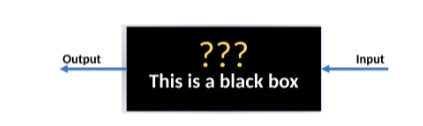
\includegraphics[width=0.75\textwidth]{images/black_box.png}}
  \caption{Blackbox Optimization}
  \label{fig:black_box}
\end{figure}
